\graphicspath{{chapters/chp1/graphics/}}


\title{Growth and Remodelling Package in FEniCSx}

\author{Karl Munthe and Henrik Finsberg and Samuel Wall and Joakim Sundnes}

\institute{K. Munthe \at Simula Research Laboratory, Oslo, Norway and \\ Department of Informatics, University of Oslo, Norway, \email{karlfredrik@simula.no}
\and
H. Finsberg \at Simula Research Laboratory, Oslo, Norway
\and
S. Wall \at Simula Research Laboratory, Oslo, Norway
\and
J. Sundnes \at Simula Research Laboratory, Oslo, Norway and \\ Department of Informatics, University of Oslo, Norway}

\maketitle
\abstract{The heart is a dynamic organ that changes its size and shape to regulate its behaviour to the demands of the body, which can change for example through body growth, exercise, the onset of a disease, or taking medication. Different models exist to try to capture various types of cardiac growth as a result of mechanical stimuli. In this manuscript we will present a framework created with FEniCSx that allows one to quickly run simulations of growth and remodelling of a unit cube with different material models and different growth laws. We present some of the simulations and compare them to the relevant literature in the field. \added{All the code can be found at \url{https://github.com/karlfm/Growth-and-Remodeling-in-FEniCSx}}}
\vspace{12pt}
\section{Introduction}
In classical continuum mechanics one normally studies the mechanics of bodies where mass\replaced{, linear momentum, angular momentum, and energy are conserved properties}{is a conserved property} conserved property. This has been extremely successful and is the bedrock for traditional engineering disciplines, but it does not accurately capture aspects of how living organisms change with respect to their environment. One of the unique features of biological material is its ability to grow by adding or removing mass. Understanding how biological matter grows and what triggers it to start or stop is important, not only to understand normal growth and development, but also when and how growth may become non-compensatory and drive disease.\par It has been known for a long time that the growth of a body is regulated at least in part by the forces applied to it \citep{Hsu1968}. This understanding has led to the formulation of growth laws that link growth and remodeling to local stress or strain. 
\section{Methods}
\subsection{Continuum Mechanics}
Consider a solid body that is continuously and smoothly deforming from one configuration to another, and denote the initial configuration (also called the reference configuration) as $\mathcal{M}$ and the current configuration $\mathcal{N}$. We denote a point in $\mathcal{M}$ with uppercase letters $\mathbf{X} = (X, Y, Z)$ and a point in $\mathcal{N}$ with lowercase letters $\mathbf{x} = (x, y, z)$\footnote{Apart from the letters $X$, $Y$, and $Z$, all upper case letters represent tensors.}. A point in $\mathcal{M}$ can be mapped to a point in $\mathcal{N}$ by a motion, $\phi(\mathbf{X}): \mathbf{X} \rightarrow \mathbf{x}$, which is a diffeomorphism. We can map a vector from the reference configuration to the current configuration via the pushforward of $\phi$, which is commonly denoted by $\mathbf{F}$ and is referred to as the deformation gradient, computed as $\partial\phi/\partial\mathbf{X} = \partial\mathbf{x}/\partial\mathbf{X}$. The displacement field $\mathbf{u} = \mathbf{x} - \mathbf{X}$ is a vector field describing the displacement of each point $\mathbf{X}$ in the reference configuration to its location $\mathbf{x}$ in the deformed configuration. \par 
The tensor $\mathbf{F}^\top\mathbf{F}$ is denoted as $\mathbf{C}$ and referred to as the right Cauchy-Green deformation tensor. Most models of the heart assume that it is hyperelastic, meaning that deformations of the material conserve its energy. If one wants to model growth of the tissue, one needs to incorporate a plastic deformation. This is commonly done with a multiplicative split, 
\begin{equation}
\label{eq: multiplicative split}
    \mathbf{F} = \mathbf{F}_e\mathbf{F}_g,
\end{equation}
where $\mathbf{F}_e$ is the elastic deformation and $\mathbf{F}_g$ is the plastic deformation that represents growth. The mulitplicative split of elastic and plastic deformations was originally motivated by the study of large deformations and was first used by \citep{Kondaurov1987}, \citep{Takamizawa1990}, and \citep{Rodriguez1994} to study growth and remodelling of biological tissue. \par 
\added{One interpretation of \ref{eq: multiplicative split} is that the material first deforms by $\mathbf{F}_g$ in a way that does not cause stress, but might cause incompatibilites in the form of discontinuities or overlapping material. The deformation described by $\mathbf{F}_g$ leads to an unphysical intermediate configuration, which is then deformed by $\mathbf{F}_e$} \deleted{Then it deforms by $\mathbf{F}_e$}in a way that removes the unphysical characteristics that occurred from $\mathbf{F}_g$, but adds residual stress. \added{Sufficient conditions for the existence of intermediate configurations such as $\mathbf{F}_g$ are discussed in \cite{Goodbrake2021}}. We assume that $\mathbf{F}_e$ is hyperelastic such that we can obtain the first Piola–Kirchhoff stress tensor by differentiating a strain energy function, $\Psi$
\begin{equation}
\label{eq: stress}
    \mathbf{P} = \frac{\partial\Psi}{\partial \mathbf{F}_e},
\end{equation}
which we use to solve the conservation of momentum equation,
\begin{equation}
\label{eq: conservation of momentum}
    \nabla\cdot\mathbf{P} = 0.
\end{equation}
Solving (\ref{eq: conservation of momentum}) will give a displacement field which is used to update the growth tensor, $\mathbf{F}_g$, via either the stress or strain tensor, resepctively called stress based and strain based growth. It is common to express the growth tensor in terms of fiber, crossfiber, and normal directions 
\begin{equation*}
    \mathbf{F}_g^\mathrm{inc} = F^\mathrm{inc}_{g,f}\mathbf{e}_f\otimes \mathbf{e}_f + F^\mathrm{inc}_{g,c}\mathbf{e}_c\otimes \mathbf{e}_c + F^\mathrm{inc}_{g,n}\mathbf{e}_n\otimes \mathbf{e}_n.
\end{equation*}
where $F^\mathrm{inc}_{g, i}$ for  $i = \{f, c, n\}$ are functions of either the stress or strain. The total deformation is obtained by 
\begin{equation*}
    \mathbf{F}_g^{i + 1} = \mathbf{F}_g^i\mathbf{F}_g^\mathrm{inc},
\end{equation*}
where the initial growth tensor, $\mathbf{F}_g^0$, is set to the identity tensor. Finally, the equations are then furnished with boundary conditions that make them well-posed. Using homogenous boundary conditions, the system of equations becomes
\begin{equation} \label{eq: system of equations}
\begin{aligned}
    \mathbf{F} & = \mathbf{F}_e\mathbf{F}_g, && \text{in } \mathcal{M}\\
    \nabla\cdot\mathbf{P} & = 0 && \text{in } \mathcal{M} \\
    \mathbf{P}\cdot \nu & = 0 && \text{on } \partial\mathcal{M}_N \\
    \mathbf{P} & = 0 && \text{on } \partial\mathcal{M}_D
\end{aligned}
\end{equation} 
where $\nu$ is a normal vector, $\partial\mathcal{M}_N$ amd $\partial\mathcal{M}_D$ denote the boundaries which are prescribed Neumann and Dirichlet boundary conditions respectively. For further information about continuum mechanics we recommend \citep{Marsden1983} and \citep{Holzapfel2002}, and for further information about growth and remodelling we recommend \citep{Goriely2017} and \citep{Yavari2010}.

\subsection{Numerical Implementation And Experiments}
For ease implementation we use a \replaced{nearly}{weakly} incompressible hyperelasticity stress tensor, so (\ref{eq: stress}) becomes
\begin{equation*}
    \mathbf{P} = \frac{\partial }{\partial \mathbf{F}_e}(\Psi_\text{iso}(\mathbf{I}_1, \mathbf{I}_2) + \Psi_\text{vol}(\mathbf{I}_3))
\end{equation*}
where $\Psi_\text{iso}$ and $\Psi_\text{vol}$ are the isochoric (distortional) and volumetric (dilational) parts of the strain energy function, and $\mathbf{I}_1$, $\mathbf{I}_2$, and $\mathbf{I}_3$ are the first three principle invariants of $\mathbf{C}$. To decouple the energy stored in the body as a result of volume preserving deformation and non-volume preserving deformation, we set $\mathbf{\bar{F}}_e = \mathbf{F}_eJ^{-1/3}$, whose determinant is equal to the identity tensor. $\mathbf{\bar{C}}$ is then used in $\Psi_\text{iso}$ and is calculated as $\mathbf{\bar{C}} = \mathbf{\bar{F}}_e^\top \mathbf{\bar{F}}_e$. Now, $\partial\Psi_\text{iso}/\partial \mathbf{F}_e \neq 0$ only if volume preserving deformation occurs, and $\partial\Psi_\text{vol}/\partial \mathbf{F}_e \neq 0$ only if non-volume preserving deformation occurs (see chapter 6 of \cite{Holzapfel2002} for more details). For example, one might use $\Psi_\text{iso} = w_1\left(\tr\mathbf{\bar{C}} - 3\right)$, and $\Psi_\text{vol} = w_2(J-1)^2$, where $J$ is the determinant of $\mathbf{F}_e$, and $w_1$, and $w_2$ are some scalar values. For the strain energy function, we used a \replaced{nearly}{weakly} incompressible neo-Hookean model
\begin{equation*}
    \Psi = \mu\Psi_\text{iso} + \kappa\Psi_\text{vol}.
\end{equation*}\par 
\added{Algorithm \ref{alg:growth_deform} shows the algorithm used for strain based growth. For stress based growth, you would update the stress tensor rather than the strain tensor, and for additatve growth laws, you would add the cumulative and incremental growth tenors instead of multiplying them together.}
\begin{algorithm} 
    \caption{Growth tensor and elastic strain tensor are updated as shown. Note that the growth tensor, $\mathbf{F}_\mathrm{g}^{i + 1}$ is updated by recursively multiplying it with the incremental growth tensor, $\mathbf{F}_g^\mathrm{inc}$. Both $\mathbf{F}_\mathrm{e}$ and $\mathbf{F}_g^\mathrm{inc}$ are dependent on $\mathbf{u}$.}\label{alg:growth_deform}
    \SetAlgoLined
    \For{i = 0 \KwTo N}{
        $\mathbf{u}$ = Solve (\ref{eq: system of equations})\;
        $\mathbf{E}_\mathrm{e}^{i + 1} = (\mathbf{F}_\mathrm{e}^\top \cdot \mathbf{F}_\mathrm{e} - \mathbf{I})/2$\;
        $\mathbf{F}_\mathrm{g}^{i + 1} = \mathbf{F}_\mathrm{g}^i * \mathbf{F}_g^\mathrm{inc}$\;
    }
\end{algorithm} 
\subsection{Solving Growth Laws on the Unit Cube}
\label{subsec: experiments}
% We will now walk through how we solve a basic growth problem for the unit cube with coordinates $(x, y, z)$, where each component ranges from 0 to 1. In other words, $\mathcal{N} = (0, 1)^3$. 
In the literature of growth and remodelling it is common to refer to the fiber direction, crossfiber direction, and the normal direction, which create a natural orthonormal basis to describe growth. In the simulations we have run we have aligned the $x$-axis with the fiber direction and the $y$-, and $z$-axis are the crossfiber and radial direction. To be consistent with the literature we will use $\mathbf{e}_f$, $\mathbf{e}_c$, and $\mathbf{e}_n$ to denote the unit vectors in the $(x, y, z)$ directions respectively.  \par
\emph{Boundary conditions:} We set the following boundary conditions
\begin{align*}
    u &= \begin{cases}
        0, & x = 0 \\
        u_D, & x = 1
    \end{cases} \\
    v &= 0, \qquad \ y = 0 \\
    w &= 0, \qquad \ z = 0
\end{align*}
where $u$, $v$, and $w$ are the displacement in the $x$, $y$, and $z$ direction respectively. $u_D$ is a Dirichlet boundary condition that specifies how much the body is displaced. 
\par
\emph{Constructing the weak form}: We multiply \ref{eq: conservation of momentum} by a test function, which we set to be in the same function space as $\mathbf{u}$, and for every subdomain $\Omega \subseteq \mathcal{M}$ the divergence of stress must equal zero. By applying integration by parts, we obtain
\begin{align*}
    \int_\Omega(\nabla\cdot\mathbf{P})\cdot\eta d\mathbf{X} &= 0 \\
    \int_\Omega \mathbf{P} : \nabla\eta d\mathbf{X} &= \int_{\partial\Omega}\mathbf{P}\cdot\eta \cdot \nu dA.
\end{align*}
\replaced{Since we are using test functions, $\eta$, that vanish on $\partial_D\mathcal{M}$, and the normal component of $\mathbf{P}$ is zero on $\partial_N\mathcal{M}$ we can set the boundary integral to zero. }{Since we are using Dirichlet boundary conditions, $\mathbf{P} = 0$ on the boundary of $\mathcal{N}$}. Additionally, since this must hold for any subdomain $\Omega \subseteq \mathcal{M}$, it must be true for the integrand. The conservation of momentum equation thus reduces to
\begin{equation}
\label{eq: weak conservation of momentum}
    \mathbf{P} : \nabla\eta = 0,
\end{equation}
which is solved using FEniCSx.
\par
\emph{Iteratively solving the conservation of momentum}: We now solve (\ref{eq: weak conservation of momentum}) for the displacement $\mathbf{u}$, which we can use to compute all the necessary variables. We use a second order, continuous, Lagrange elements to approximate $\mathbf{u}$ and a first order, discontinuous, Lagrange elements to approximate $\mathbf{F}_e$ and $\mathbf{F}_g$. $\mathbf{F}_g$ is initially set to be the identity tensor. \par
\emph{Numerical experiments:} We ran one simulations where we stretched a unit cube by 10\% in the fiber direction (along the $x$-axis), which we will refer to as the stretch simulation, and another simulation where we compressed a unit cube by 10\% in the fiber direction (along the $x$-axis), which we will refer to as the compression simulation. $u_D = 0.1$ and $-0.1$ for the stretch and compression simulation respectively. In the stretch simulation $F_{g,c,\mathrm{max}}$ was set to 1.2 and 0.8 in the compression simulation. We set $\mu = 15$ kilo Pascals and $\kappa = 100$ kilo Pascals.
\subsection{The different growth models}
\label{sub:different models} 
In this paper we compare five growth models which we have taken from \citep{Taber1998}, \citep{Kroon2009}, \citep{Goktepe}, and \citep{Kerckhoffs2012}. The growth models are given in table \ref{tab:growth models} where LT2 is from \citep{Taber1998}, KFR is from \citep{Kroon2009}, GEG and GCG are from \citep{Goktepe} and KOM is from \citep{Kerckhoffs2012}. Each growth model had a set point that either determined the homeostatic level of stress, stretch, or strain. When the stress, stretch, or strain reaches the set point, then growth will cease to occur. If this does not happen, the body will grow indefinitely, which we call runaway growth. We used the same variables as they were given in the original papers, except for the \replaced{GCG}{$GCG$}, where we scaled the variables to more accurately fit with the shear modulus used here. The values are tabulated in table \ref{tab:parameters}.
\newgeometry{right=1cm, left=1cm}%,right=1cm,top=1cm,bottom=1cm}
\begin{table}
\centering
\renewcommand{\arraystretch}{5}
\begin{tabular}{|c||c|c|c|}
\hline \hline
 & $F_{g,f}^{i+1}$ & $F_{g,r}^{i+1}$ & $F_{g,c}^{i+1}$ \\
\hline \hline
LT2 & $\displaystyle F_{g,f}^i\left(\frac{\sigma_{\theta p} - \sigma_{p,0}}{T\sigma_{p,0}} + 1\right)$ & $\displaystyle F_{g,r}^i\left(\frac{\sigma_{\theta a} - \sigma_{a,0}}{T\sigma_{a,0}} + 1\right)$ & $\displaystyle 1$ \\
\hline
KFR & $\displaystyle F_{g,f}^i(\beta(\sqrt{2 E_{ff} + 1} - 1 - s_\mathrm{hom}) + 1)^{1/3}$ & $\displaystyle F_{g,r}^i(\beta(\sqrt{2 E_{ff} + 1} - 1 - s_\mathrm{hom}) + 1)^{1/3}$ & $\displaystyle F_{g,c}^i(\beta(\sqrt{2 E_{ff} + 1} - 1 - s_\mathrm{hom}) + 1)^{1/3}$ \\
\hline
GEG & $\displaystyle \frac{1}{\tau}\left(\frac{F_{g,f,\mathrm{max}} - F_{g,f}^i}{F_{g,f,\mathrm{max}} - 1}\right)^\gamma(F_{e, f}^i - \lambda^\text{crit}) + F^i_{g, f}$ & $\displaystyle 1$ & $\displaystyle 1$ \\
\hline
GCG & $\displaystyle 1$ & $\displaystyle  \frac{1}{\tau}\left(\frac{F_{g,c,\mathrm{max}} - F_{g,c}^i}{F_{g,c,\mathrm{max}} - 1}\right)^\gamma(\tr(\mathbf{M}) - p^\mathrm{crit}) + F^i_{g, c}$ & $\displaystyle 1$ \\
\hline
KOM & $\displaystyle \begin{cases}
        F_{g,f}^{i}k_{ff}\frac{f_\mathrm{ff, max}\Delta t_\text{growth}}{1 + \exp(-f_f(s_\mathrm{l}-s_{l,50}))} + 1, \qquad s_\mathrm{l} \geq 0\\
        F_{g,f}^{i}\frac{-f_\mathrm{ff, max}\Delta t_\text{growth}}{1 + \exp(f_f(s_\mathrm{l}+s_{l,50}))} + 1, \qquad s_\mathrm{l} < 0
    \end{cases} $ & $\displaystyle \begin{cases}
        F_{g,c}^{i}\sqrt{k_{cc}\frac{f_{cc,\mathrm{max}}\Delta t_\text{growth}}{1 + \exp(-c_\mathrm{f}(s_\mathrm{t}-s_{t,50}))} + 1}, \qquad s_\mathrm{t} \geq 0\\
        F_{g,c}^{i}\sqrt{\frac{-f_{cc,\mathrm{max}}\Delta t_\text{growth}}{1 + \exp(c_\mathrm{f}(s_\mathrm{t}+s_{t,50}))} + 1}, \qquad s_\mathrm{t} < 0 
    \end{cases} $ & $\displaystyle \begin{cases}
        F_{g,c}^{i}\sqrt{k_{cc}\frac{f_{cc,\mathrm{max}}\Delta t_\text{growth}}{1 + \exp(-c_\mathrm{f}(s_\mathrm{t}-s_{t,50}))} + 1}, \qquad s_\mathrm{t} \geq 0\\
        F_{g,c}^{i}\sqrt{\frac{-f_{cc,\mathrm{max}}\Delta t_\text{growth}}{1 + \exp(c_\mathrm{f}(s_\mathrm{t}+s_{t,50}))} + 1}, \qquad s_\mathrm{t} < 0 
    \end{cases} $ \\
\hline
\end{tabular}
\caption{$F_{g,f}$, $F_{g,r}$, $F_{g,s}$ for each of the five models. The parameters $T$, $\beta$, $\tau$, and $\Delta t$, simply determine the rate of growth and can be tuned to \replaced{match}{math} the growth rate of data obtained from experiments.}
\label{tab:growth models}
\end{table}
\restoregeometry
\begin{table}[htbp]
    \centering
    \begin{tabular}{|l|l|}
    \hline
    \textbf{Model} & \textbf{Parameters} \\
    \hline
    \textbf{LT2} &   $\sigma_{a,0} = 30, \sigma_{p,0} = 3, T = 10^{-4}$ \\ \hline
    \textbf{KFR} &  $s_\mathrm{hom} = 0.13, \beta = 10^{-2}$ \\ \hline
    \textbf{GEG} &  $F_{g,f,\mathrm{max}}=1.5, \lambda^\mathrm{crit}=1.01,\gamma = 2, \tau = 10^2$ \\ \hline
    \textbf{GCG} &  $F_{g,c,\mathrm{max}}=1.2$ and $0.8$,  $p^\mathrm{crit}=0.12, \gamma = 2, \tau = 10^4$ \\ \hline
    \textbf{KOM} &  $f_\mathrm{ff,max} =0.31, f_f = 150, s_{l50} = 0.06, F_{ff50} = 1.35, f_{l,\mathrm{slope}} = 40, f_\mathrm{ff,max} = 0.1$ \\
        & $c_\mathrm{f} = 75, s_\mathrm{t50} = 0.07, F_\mathrm{cc50} = 1.28, c_\mathrm{th,slope} = 60, E_{ff,\mathrm{set}} = 0, 
        E_\mathrm{cross,\mathrm{set}} = 0, \Delta t = 10^{-2}$ \\ \hline
    \end{tabular}
    \caption{Model parameters for the growth models.}
    \label{tab:parameters}
\end{table}
In LT2, $\sigma_{p,0}$ and $\sigma_{a,0}$ are set points for the passive and active fiber stress at equilibrium, and $\sigma_{\theta p}$ and $\sigma_{\theta a}$ are the active and passive fiber stresses. In the simulations we have run, we have decomposed $\sigma$ such that the active component is oriented along the fiber direction, and the passive component is oriented along the crossfiber direction. For KFR, $s_\mathrm{hom}$ is the strain set point. For GEG and GCG, $F_{g,f,\mathrm{max}}$ and $F_{g,c,\mathrm{max}}$ is the maximum amount of growth allowed to occur. $\mathbf{M}$ is the Mandel stress, which is defined as 
\begin{equation*}
    \mathbf{M} = \mathbf{F}^\top \mathbf{P}
\end{equation*}
and $p^\mathrm{crit}$ is the stress set point. $\lambda^\text{crit}$ is the strain set point. For KOM, $k_{ff}$ and $k_{cc}$ are defined as
\begin{align*}
    k_{ff} &= \frac{1}{1 + \exp(f_\text{length,slope}(\mathbf{F}_{g,ff}^i - F_{ff,50}))} \\
    k_{cc} &= \frac{1}{1 + \exp(c_\text{thickness,slope}(\mathbf{F}_{g,cc}^i - F_{cc,50}))}
\end{align*}
and $s_\mathrm{l}$, and $s_\mathrm{t}$ are defined as
\begin{align*}
    s_\mathrm{l} &= \max(E_{ff}) - E_{ff, \mathrm{set}} \\
    s_\mathrm{t} &= \min(E_\text{cross, max}) - E_\mathrm{cross, set}
\end{align*}
where $E_{ij}$ is the Lagrange strain tensor, and $E_{ff}$ is the strain in the fiber direction, and $E_\text{cross, max}$ is the maximum algebraic maximum principle strain of the matrix (see \citep{Witzenburg2018})
\begin{equation*}
    E_\text{cross} = \begin{pmatrix}
        E_{cc} & E_{cr} \\
        E_{rc} & E_{rr}
    \end{pmatrix}
\end{equation*}
and $E_{ff, \mathrm{set}}$ and $E_\mathrm{cross, set}$ are set points. \par
\deleted{In the simulations run, LT2 displayed runaway growth as was also observed in the simulations run in }\citep{Witzenburg2018}. Growth stops for the LT2 model when \begin{equation}
\label{eq: LT2 equilibrium}
    \frac{\sigma_{\theta} - \sigma_{0}}{\sigma_{0}} = T\left(\frac{1}{F_{g}^i} - 1\right).
\end{equation}
\deleted{which was not satisfied in our simulations or in the simulations run by} \citep{Witzenburg2018}. Since $F_g^i$ is dependent on $\sigma$ which in turn is nonlinearly dependent on $F_g^{i-1}$ it is not straightforward to know under what conditions \ref{eq: LT2 equilibrium} will be satisfied. For GCG and GEG, the simulations show that they are forced to stop either when the stretch or stress reaches the growth limit or when the maximal allowed growth is reached. For KOM, since $k_{cc}$ and $k_{ff}$ are logistic functions, the growth is bounded from above and below inhibiting runaway growth. Finally, for KFR, it does not appear obvious that it will not obtain runaway growth, but other simulations setups that were tested did result in runaway growth, even though the one we present here does not.
\section{Results}
The data we collected from the two experiments (see bottom of section \ref{subsec: experiments}) were the the stretch and growth that occurred in the middle of the cube. The results are depicted in figures \ref{fig:10p_stretch} and \ref{fig:10p_compression}. The top row of each figure displays the fiber and crossfiber components of the growth tensor, $F_g$, and the bottom row displays the fiber and crossfiber components of the elastic deformation tensor $F_e$. Increasing $\kappa$ did not yield qualitatively different results. \par
First, we note that LT2 displayed runaway growth, as was also found in \citep{Witzenburg2018}. GCG seems to be converging to $F_{g,c,\mathrm{max}}$, and GEG seem to have converged because it reached $\lambda^\text{crit}$. The reason GCG is growing oppositely compared to GEG is probably because GEG was created to model growth triggered by volume overload while GCG was created to capture growth triggered by pressure overload. KFR grew an equal amount in each direction, and stabilized. It is not clear under what conditions KFR should be stable because $s_\mathrm{hom}$ is the same in each direction. When we ran simulations with other boundary conditions, it was not stable. The KOM model was stable for many different types of boundary conditions, but is the most computationally expensive model to run.\par 
The package makes it easy to run similar simulations with different material models and different boundary conditions, but we do not have the space to display the results here. \par
\begin{figure}[h]
    \centering
    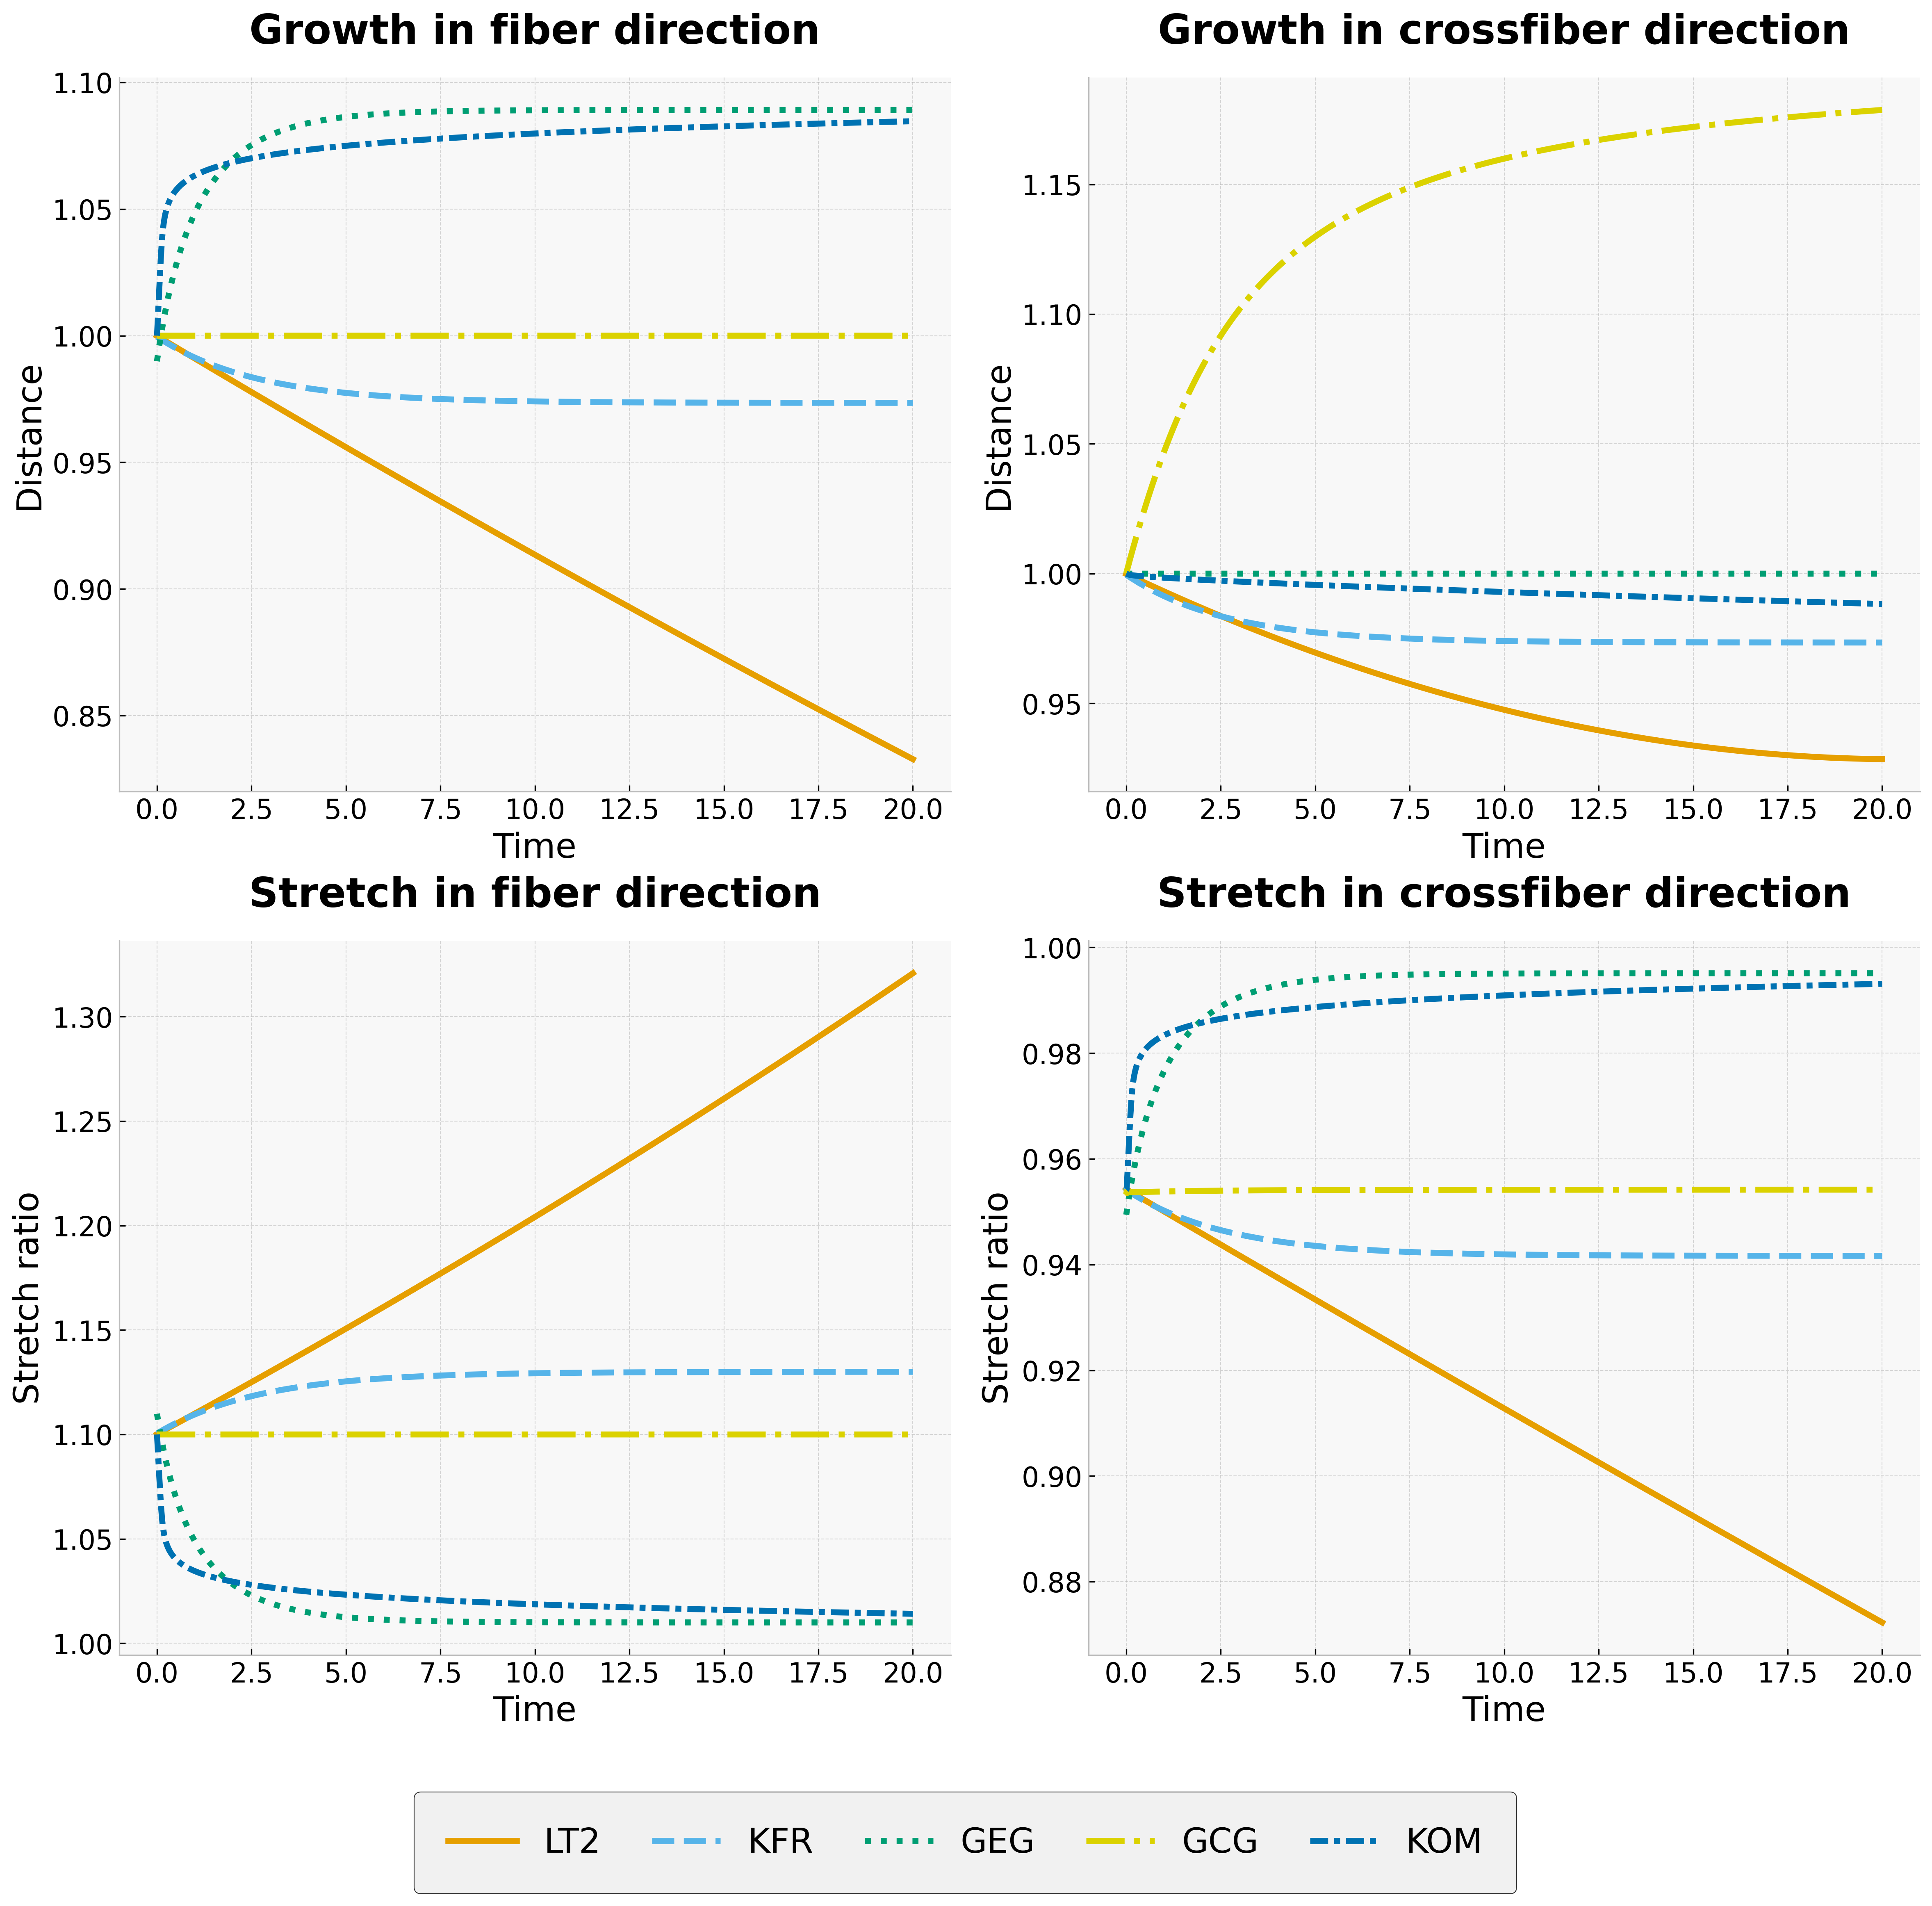
\includegraphics[width=\textwidth]{10p_stretch_fiber2.png}
    \caption{Growth and stretch predicted by a 10\% stretch in the fiber direction. The runaway growth in LT2 was also reported in \citep{Taber1998}.}
    \label{fig:10p_stretch}
\end{figure}
\begin{figure}[h]
    \centering
    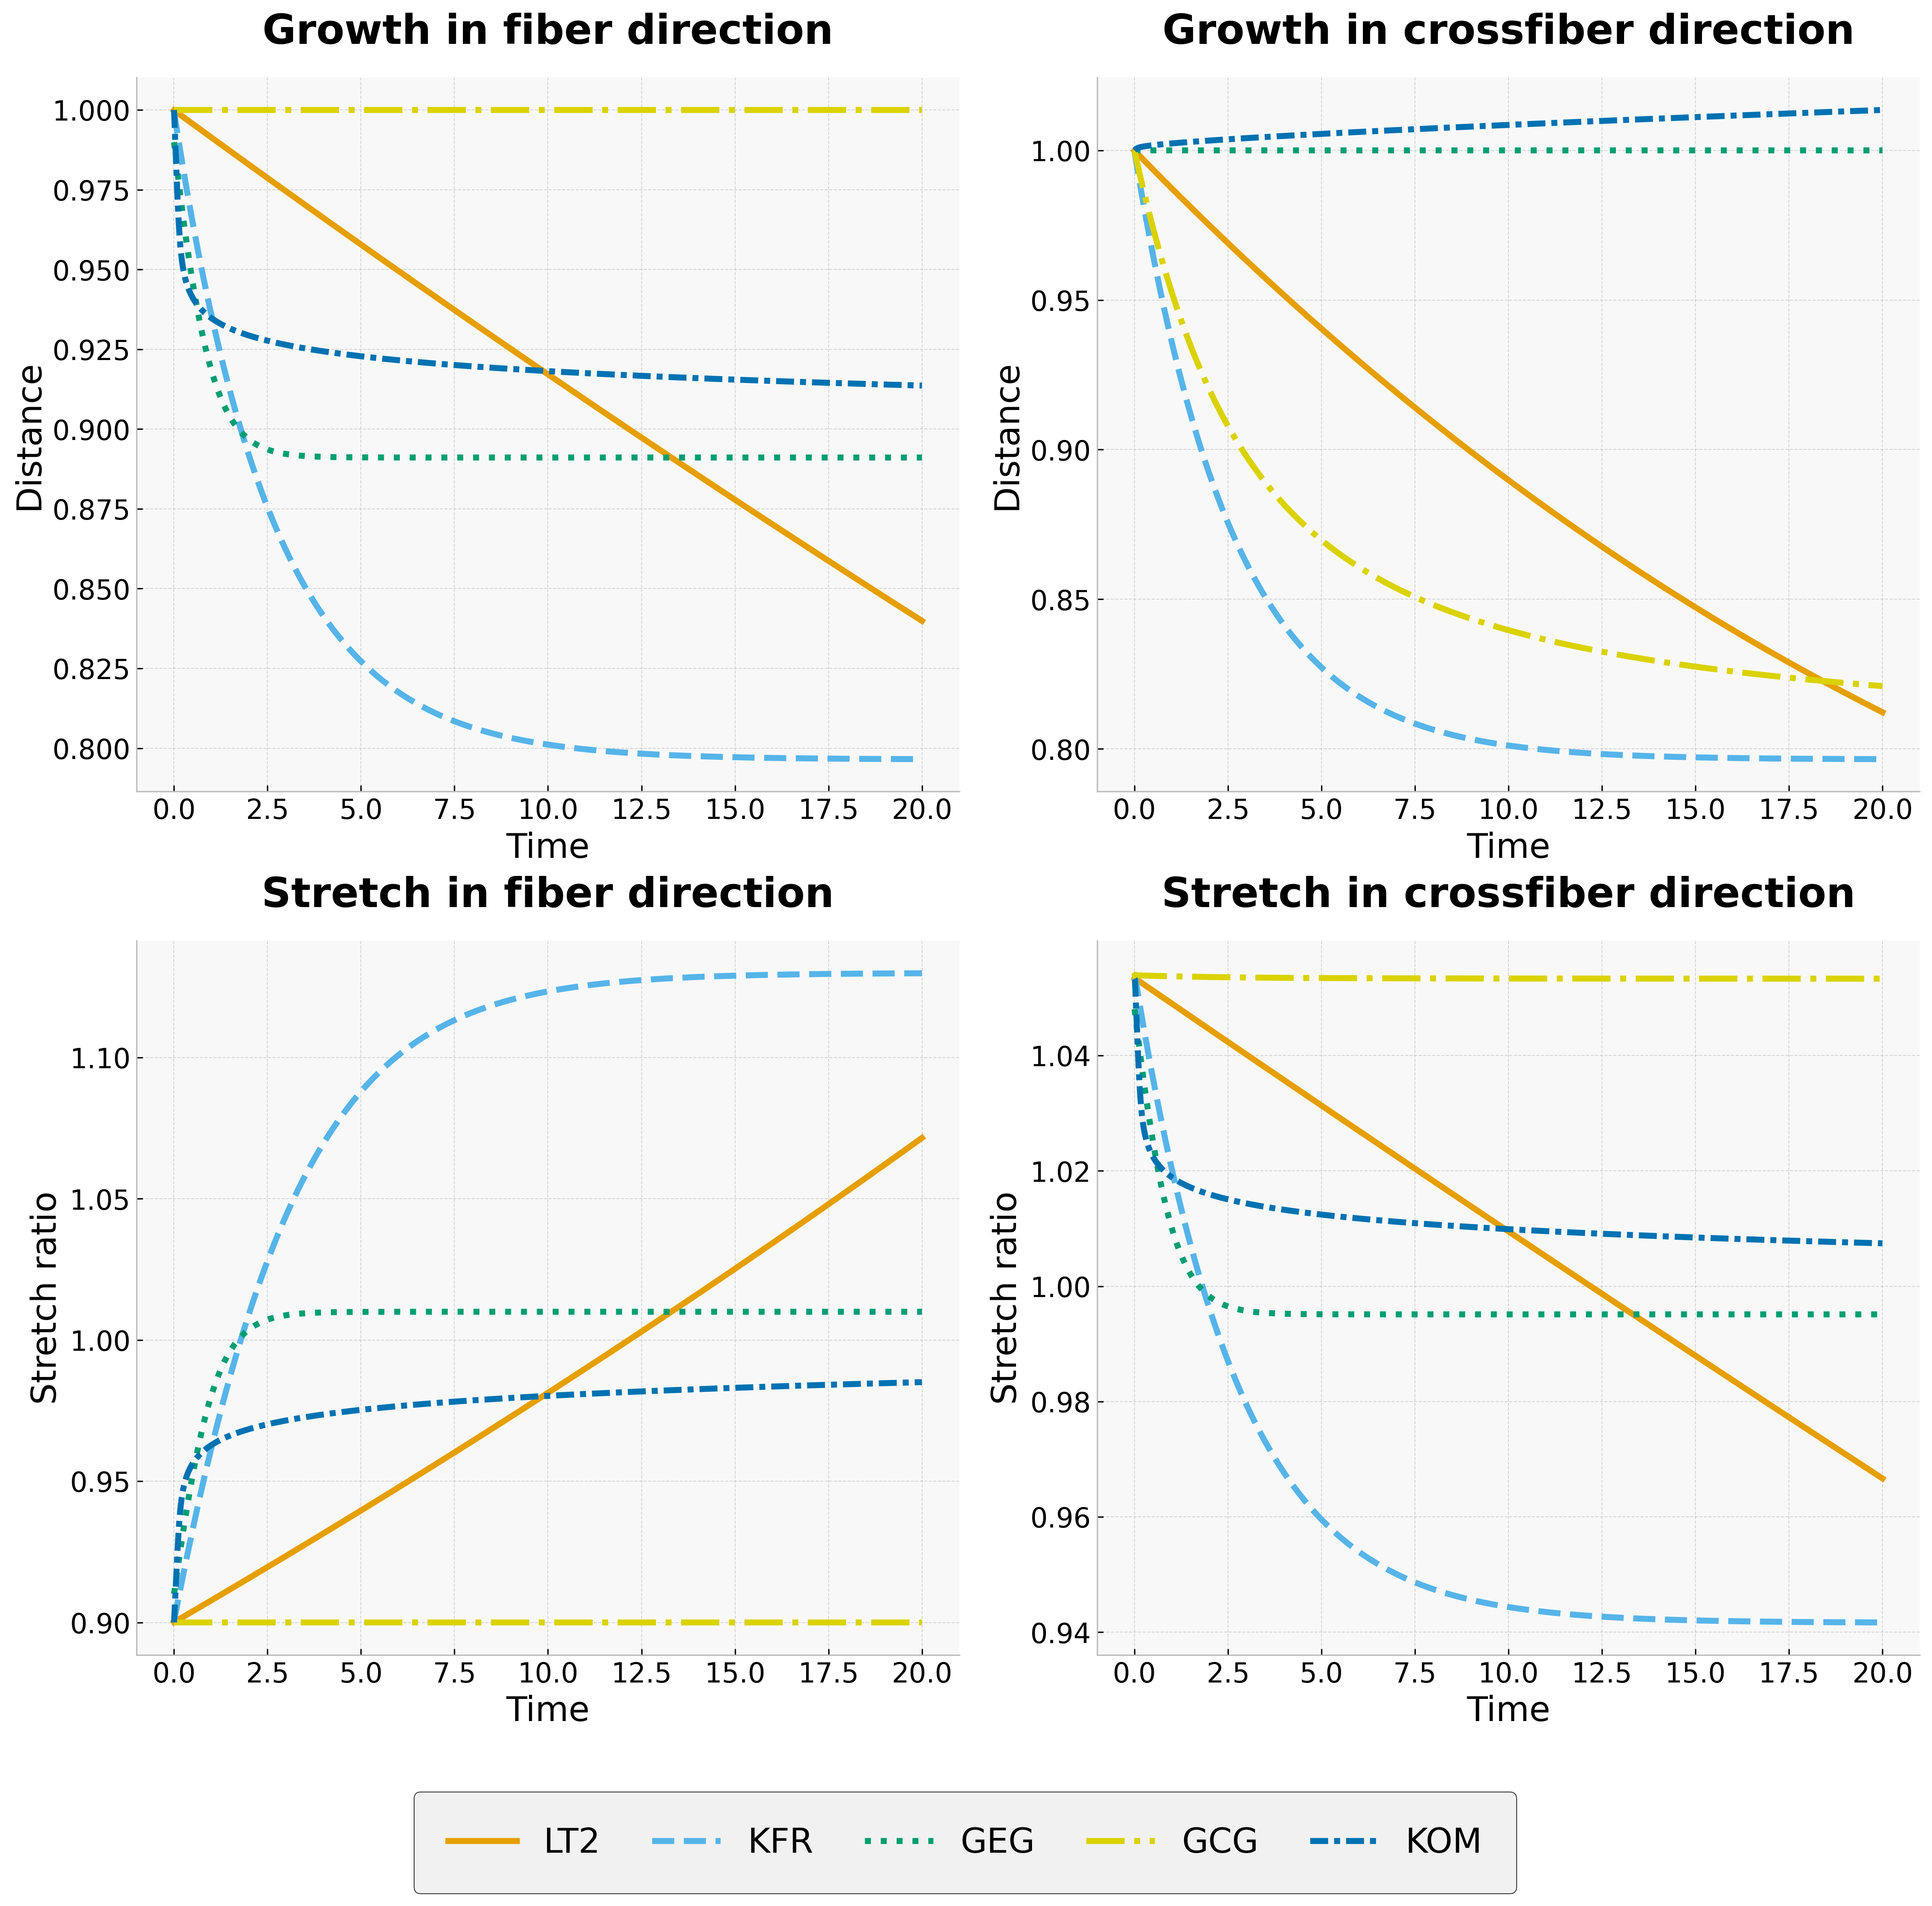
\includegraphics[width=\textwidth]{10p_compression_fiber2.png}
    \caption{Growth and stretch predicted by a 10\% compression in the fiber direction. For the models that converge, these results make intuitive sense; as time increases the growth appraoches the stretched state and the stretch (which is solely computed from $\mathbf{F}_e$) approaches 1.}
    \label{fig:10p_compression}
\end{figure}    
\section{Conclusion and future work}
We have implemented a general growth and remodelling framework using the FEniCSx program in Python. The goal is to easily change material models and growth models. Hopefully this will allow researchers to compare their models with other models in the field. Future work will include implementing more complex geometries, more growth laws, and more material models. \added{The models we have used in this paper are not derived from the dissipation equation but are instead phenomenologically derived growth laws and future work should investigate whether or not they satisfy the laws of thermodynamics. Another avenue of future research would be to look into constrained mixture models which model how changes in the various constituents influence the characterstics of the tissue.} \deleted{Specifically, w}\added{W}e wish to add models that have more mathematically sophisticated stopping criteria, such as the ones developed by Erlich et al. \citep{Erlich2023} uses an energy penalty to construct a stopping criteria and \citep{Erlich2024} looks into how curvature\footnote{The intrinsic three dimensional curvature, not the two dimensional curvature of the surface of the body.} in the reference configuration could be used as a stopping criteria. Future work will also implement the growth models on geometries with fibers. We tried running the models on various fiber orientations and found them extremely sensitive to fibers that varied throughout the domain. Preliminary results indicate that some of the models do not converge to a steady state for relatively small perturbations of the variables or if the fibers are not well aligned with the body. We hope to quantify this in a future paper. \par
When this package is further developed we hope to add to to the Pulse\footnote{https://github.com/finsberg/fenicsx-pulse} package. Hopefully, this will allow us to combine a circulation model with a growth model which will enable us to more accurately describe cardiac growth and remodelling phenomena. \par
The models we compared have been developed to capture different aspects of growth and were tuned to be used on different material models, so an apples-to-apples comparison might not be fair. Furthermore, the growth models we have used are not taking into account residual stresses that exist within the material before growth occurs. \par
Finally, experimental data is needed to verify which models are accurate or capture the correct phenomena of growing cardiac tissue.
% \newpage
\bibliographystyle{spbasic}
\bibliography{chapters/chp1/bibliography.bib}
% \printbibliography
% \end{document}
